

\actTitle{Worksheet 1.8}



\noindent \textbf{Instructions:}  Work together in groups of  3 or 4 to complete the following problems.

Student goals:
  \begin{itemize}
  \item Perform basic operations between functions ($+/-/*/\div$).
  \item State the correct order of operations given an algebraic expression.
  \item Compose multiple  functions.
  \item Determine the difference quotient at a point given a function.
  \end{itemize}



\begin{enumerate}
\item Given $f(x)=5x^2+2x-3$ and $g(x)=x+3$.
\begin{enumerate}
\item Determine $(f \circ g)(x)$.
\vfill


\item  Determine $(g \circ f)(x)$.
\vfill
 
 \item Determine $(f \circ g)(1)$.
 \vfill
 
 \item  Determine $(g \circ f)(1)$.
 
 \vfill
 \end{enumerate}

\clearpage

\item Given $f(x)=x^2$ and $g(x)=\sqrt{x}$.
\begin{enumerate}
\item Determine the domains of $f(x)$ and $g(x)$.
  \vfill
\item Determine $(f \circ g)(x)$ and simplify completely.
  \vfill
\item Determine the domain of $(f \circ g)(x)$.  Keep in mind that the
  domain of a function is the collection of $x$-values that can be
  plugged into the function.
  \vfill
\item  Determine $(g \circ f)(x)$ and simplify completely.
  \vfill
\item Determine the domain of $(g \circ f)(x)$.
  \vfill
\item What do you notice about $(f \circ g)(x)$ and $(g \circ f)(x)$?
  What do you notice about their domains?  Does the domain of the
  inside function affect the domain of function composition?
  \vfill
\end{enumerate}




\vfill

\clearpage 

\item Let $f(x)=x^2-1$, $g(x)$ be given by the graph below, and $h(x)$ be given by the table below.


\begin{minipage}[t]{.75\textwidth}
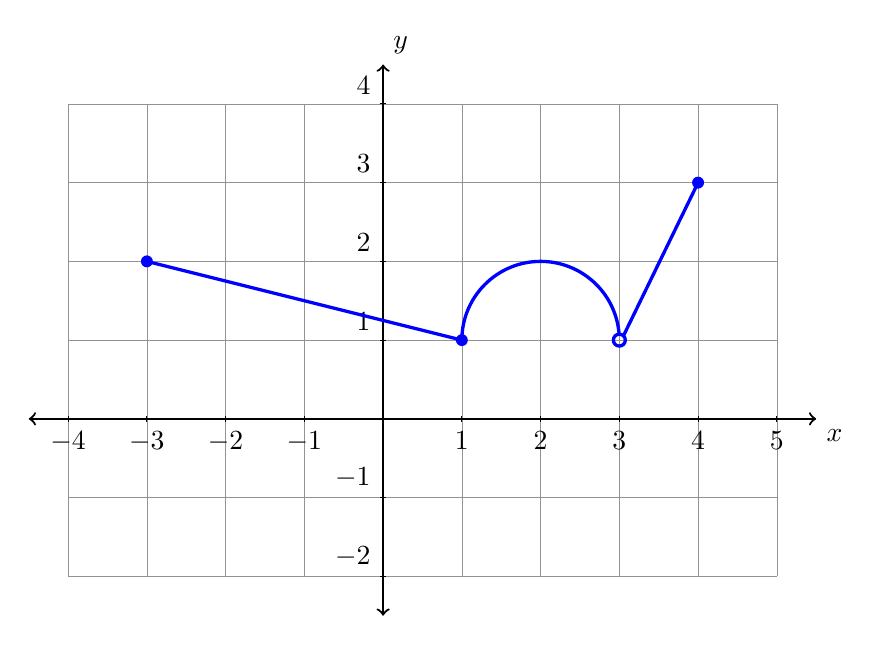
\begin{tikzpicture}[y=1cm, x=1cm,font=\sffamily,
	mydot/.style={
    circle,
    fill=white,
    draw,
    outer sep=0pt,
    inner sep=1.5pt
  }]
    %% Add a grid
    \draw[step = 1, gray, very thin,opacity=0.85] (-4, -2) grid (5, 4);
 	%% Draw the axes
	\draw[thick,<->] (-4.5,0) -- coordinate (x axis mid) (5.5,0) node[anchor = north west] {$x$};
    \draw[thick,<->] (0,-2.5) -- coordinate (y axis mid) (0,4.5) node[anchor = south west] {$y$};
    %% Label the y axis
    \foreach \y in {-2,...,-1,1,2,...,4} {
      \draw (1pt, \y) -- (-1pt, \y) node[anchor = south east] {$\y$};
    }
    %% Label the x axis
    \foreach \x in {-4,...,-1,1,2,...,5} {
      \draw (\x,1pt) -- (\x,-1pt) node[anchor = north] {$\x$};
    }
    %% Draw the function.
    \begin{scope}
         \draw[very thick,blue] (-3,2) -- (1,1);
         \draw[very thick,blue] (3.05,1.05) -- (4,3);
    %semi-circle
         \draw[very thick, blue] (1,1) arc [radius=1, start angle=180, end angle= 5];
     %parabola
     %    \draw[ultra thick, blue, domain=-5:0] plot (\x, {(-0.2)*(\x-5)*(\x+5)});
     %dots
         \fill[blue] (-3, 2) circle[radius=0.5ex];
         \fill[blue] (1,1) circle[radius=0.5ex];
         \fill[blue] (4,3) circle[radius=0.5ex];
         \draw[very thick, blue] (3,1) circle[radius=0.5ex];


    \end{scope}

    %%\node[above=0.1cm] at (-2,2 )   {\nextXValue};

  \end{tikzpicture}
\end{minipage}
%second column
\begin{minipage}[t]{.25\textwidth}
\vspace{-2in}
\begin{tabular}{|l|l|}
\hline
\textbf{$x$} & \textbf{$h(x)$} \\ \hline
-3           & 2               \\ \hline
0            & 4               \\ \hline
1            & 5               \\ \hline
3            & -6              \\ \hline
\end{tabular}
\end{minipage}







\begin{enumerate}
\item Determine the $(f\circ g)(4)$.\vfill
\item Determine the $(g\circ h)(-3)$.\vfill
\item Determine the $(h\circ f)(1)$..\vfill
\item Determine the $(g\circ f)(2)$.\vfill
\end{enumerate}


\clearpage

\item Given $f(x)=4x-9$ and $g(x)=\sqrt{x+6}$
\begin{enumerate}
\item Determine $\displaystyle\left(\frac{f}{g}\right)(x)$ and determine its domain.
\vfill
\item Determine $\displaystyle\left(\frac{g}{f}\right)(x)$ and determine its domain.
\vfill
\end{enumerate}

\item Given $f(x)=2x^2-5x+1$.  Determine the difference quotient,
  $\displaystyle \frac{f(x+h)-f(x)}{h}$.
  \sideNote{Simplify the result as much as possible.}
\vfill
\vfill

\clearpage

\item Two functions are defined by
  \begin{eqnarray*}
    \begin{array}{lcl@{\hspace{2em}}lcl}
      k(x) & = & |x|-2, & m(x) & = & 4-x^2.
    \end{array}
  \end{eqnarray*}

  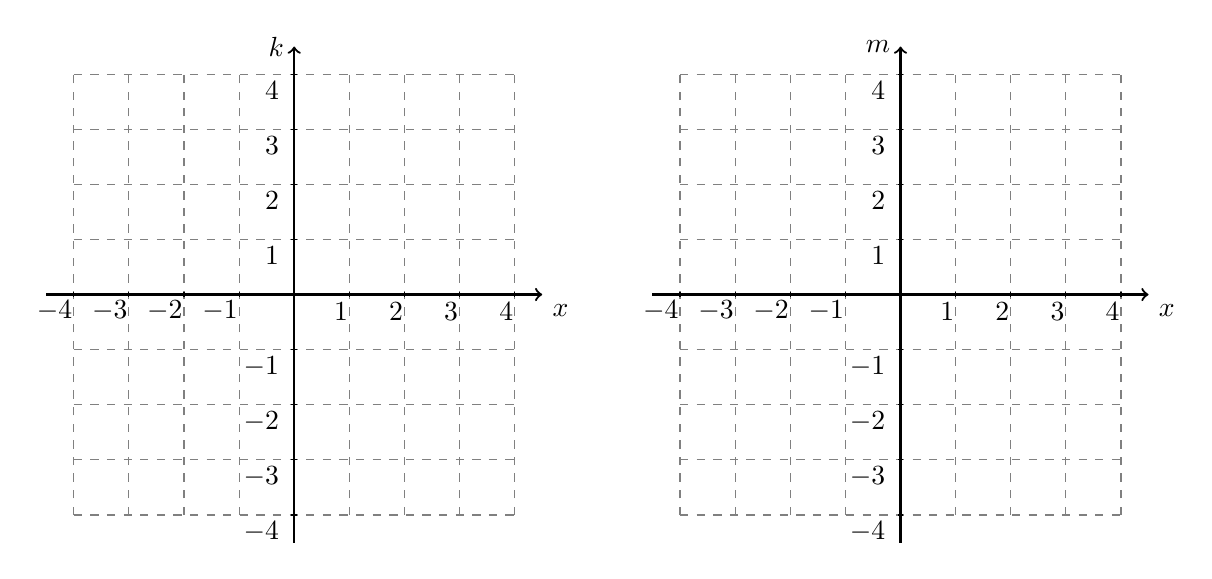
\begin{tikzpicture}[y=0.7cm, x=0.7cm,font=\sffamily]

    \begin{scope}[shift={(0,0)}]      
      %% ticks
      \draw[step = 1, gray,dashed] (-4,-4) grid (4,4);
      %% axis
      \draw[thick,->] (-4.5,0) -- coordinate (x axis mid) (4.5,0) node[anchor = north west] {$x$};
      \draw[thick,->] (0,-4.5) -- coordinate (y axis mid) (0,4.5) node[anchor = east] {$k$};
      \foreach \y in {-4,-3,-2,-1,1,2,3,4} {
        \draw (1pt, \y) -- (-1pt, \y) node[yshift=-6,xshift=-1,anchor=east] {$\y$};
      }
      \foreach \x in {-4,-3,-2,-1,1,2,3,4} {
        \draw (\x,1pt) -- (\x,-1pt) node[yshift=-5,xshift=3,anchor=east] {$\x$};
      }
    \end{scope}

    \begin{scope}[shift={(11,0)}]      
      %% ticks
      \draw[step = 1, gray,dashed] (-4,-4) grid (4,4);
      %% axis
      \draw[thick,->] (-4.5,0) -- coordinate (x axis mid) (4.5,0) node[anchor = north west] {$x$};
      \draw[thick,->] (0,-4.5) -- coordinate (y axis mid) (0,4.5) node[anchor = east] {$m$};
      \foreach \y in {-4,-3,-2,-1,1,2,3,4} {
        \draw (1pt, \y) -- (-1pt, \y) node[yshift=-6,xshift=-1,anchor=east] {$\y$};
      }
      \foreach \x in {-4,-3,-2,-1,1,2,3,4} {
        \draw (\x,1pt) -- (\x,-1pt) node[yshift=-5,xshift=3,anchor=east] {$\x$};
      }
    \end{scope}


  \end{tikzpicture}

  \begin{enumerate}
  \item Use the two axes above to make a rough sketch of both
    functions.
  \item For what values of $x$ is $k(x)=0$?
    \vfill
  \item Determine the $x$-intercepts of $k(m(x))$.
    \vfill
  \item For what values of $x$ is $k(x)$ increasing?
    \vfill
  \item Determine the values of $x$ where $k(m(x))$ is increasing.
    \vfill
  \end{enumerate}


\end{enumerate}


\hwTitle{Section 1.8}

\begin{enumerate}
\item Given $f(x)=x^2$ and $h(x)=\sqrt{-x}$.
\begin{enumerate}
\item Determine the domains of $f(x)$ and $h(x)$.
\item Determine $(f \circ h)(x)$ and simplify completely.
\item Determine the domain of $(f \circ h)(x)$.  Keep in mind that the
  domain of a function is the collection of $x$-values that can be
  plugged into the function.
\item  Determine $(h \circ f)(x)$ and simplify completely.
\item Determine the domain of $(h \circ f)(x)$.
\item Make a rough sketch of the functions $(f \circ h)(x)$ and
  $(h \circ f)(x)$ on the same axes.
\end{enumerate}

\item Two functions are given below. The graph of $h(x)$ is on
    the left, and the function $s(x)$ is defined on the right.
  
    \begin{tabular}{p{0.7\textwidth}p{0.3\textwidth}}
      \begin{minipage}{0.5\linewidth}
        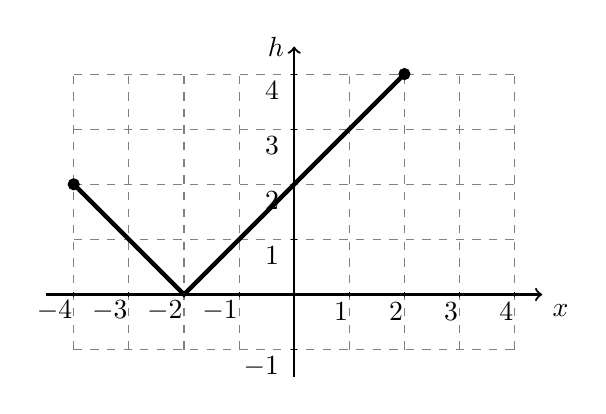
\begin{tikzpicture}[y=0.7cm, x=0.7cm,font=\sffamily]
          %% ticks
          \draw[step = 1, gray,dashed] (-4,-1) grid (4,4);
          %% axis
          \draw[thick,->] (-4.5,0) -- coordinate (x axis mid) (4.5,0) node[anchor = north west] {$x$};
          \draw[thick,->] (0,-1.5) -- coordinate (y axis mid) (0,4.5) node[anchor = east] {$h$};
          \foreach \y in {-1,1,2,3,4} {
            \draw (1pt, \y) -- (-1pt, \y) node[yshift=-6,xshift=-1,anchor=east] {$\y$};
          }
          \foreach \x in {-4,-3,-2,-1,1,2,3,4} {
            \draw (\x,1pt) -- (\x,-1pt) node[yshift=-5,xshift=3,anchor=east] {$\x$};
          }

          \draw[ultra thick] plot coordinates
          {(-4,2) (-2,0) (2,4)};


          % \draw[ultra thick,black] (0,-1) --  (4,3);
          \draw[black,fill=black]  (-4,2) circle (0.1);
          \draw[black,fill=black]  ( 2, 4) circle (0.1);
        \end{tikzpicture}
      \end{minipage}

      &
        \begin{minipage}{0.3\linewidth}
          \begin{eqnarray*}
            s(x) & = & x^2 - 4.
          \end{eqnarray*}
        \end{minipage}

    \end{tabular}
\begin{enumerate}
  \item Determine the value of $s(h(-2))$.
  \item Determine the value of $h(s(-2))$.
  \item Determine the $y$-intercepts of $h(s(x))$.
  \item Determine the $x$-intercepts of $h(s(x))$.
\end{enumerate}

\item A turtle is in a field. Initially, it is 40 meters north and 60
  meters west of the center of the field. The turtle is moving at a
  constant speed, and it moves east one meter per minute.
  \begin{enumerate}
  \item Determine a formula for the distance between the turtle and
    the center of the field given the turtle's coordinate. (You should
    only have a function of the $x$-coordinate.)
  \item Determine the value of the $x$-coordinate of the turtle's
    position at any time, $t$.
  \item Use composition to determine the distance between the turtle's
    position and the center of the field for any time, $t$.
  \item Sketch a plot of the distance as a function of time. 
  \end{enumerate}

\item Three functions, $k(x)$, $w(x)$, and $g(x)$, are given
  below. Use the functions to answer each of the questions below.

  \begin{tabular}{m{0.4\linewidth}m{0.2\linewidth}m{0.3\linewidth}}

      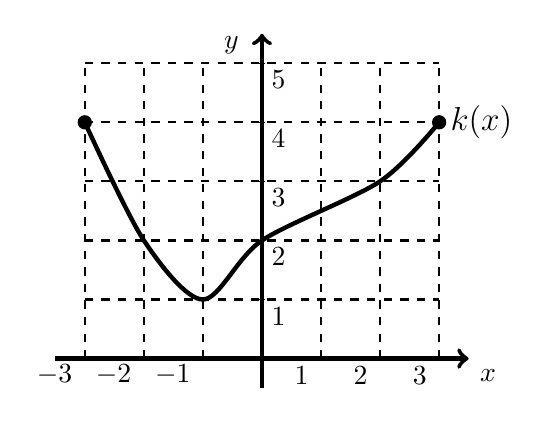
\begin{tikzpicture}[y=0.75cm, x=0.75cm,font=\sffamily]
        \begin{scope} %[shift={(0,8)}]
          %% ticks
          \draw[xstep = 1, ystep=1.0,black,dashed,thick] % very thin,opacity=0.85,
                 (-3.0,0.0) grid ( 3.0, 5.0);
             %% axis
           \draw[ultra thick,->] (-3.5,0) -- coordinate (x axis mid) (3.5,0)
                node[anchor = north west] {$x$};
           \draw[ultra thick,->] (0,-0.5) -- coordinate (y axis mid) (0,5.5)
                node[anchor = east,shift={(-0.2,-0.2)}]  {$y$};
            %% \draw[ultra thick,black] 
           \draw[ultra thick] plot [smooth] coordinates
               {(-3,4) (-2,2) (-1,1) (0,2) (2,3) (3,4) } node[anchor=west] {\large $k(x)$};
           \fill[black] (-3,4) circle [radius=0.6ex]; % Draw an open dot on the 
           \fill[black] (3,4) circle [radius=0.6ex]; % Draw an open dot on the 

           \foreach \y in {1,2,...,5} {
              \draw (1pt, \y) -- (-1pt, \y) node[yshift=-6,xshift=1,anchor=west] {$\y$};
            }
           \foreach \x in {-3,-2,-1,1,2,3} {
              \draw (\x,1pt) -- (\x,-1pt) node[yshift=-5,xshift=-1,anchor=east] {$\x$};
            }

          \end{scope}
        \end{tikzpicture}


    &

      \begin{tabular}{r|r}
        $x$ & $w(x)$ \\ \hline
        0 & -2 \\
        1 & -3 \\
        2 &  0 \\
        3 & -1 \\
        4 &  2 \\
        5 &  3
      \end{tabular}

    &

        \begin{eqnarray*}
          g(x) & = & \left\{
                     \begin{array}{lcccl}
                        x   & x & < & 0 \\ 
                       -x+3 & x & > & 0 \\ 
                     \end{array}
          \right.
        \end{eqnarray*}


  \end{tabular}

  \begin{enumerate}
  \item Determine the value of   $ {\displaystyle w(k(-1))  } $
  \item  Determine the value of   $ {\displaystyle w(g(5))  } $
  \item Determine the average rate of change of $g(x)$ from $x=-2$
    to $x=4$.
  \item  For what values of $x$ is the function $g(k(x))$ increasing?
  \end{enumerate}

\item A general quadratic function is defined by 
  \begin{eqnarray*}
    q(x) & = & a x^2 + b x + c,
  \end{eqnarray*}
  where $a$, $b$, and $c$ are constants.

  \begin{enumerate}
  \item Determine the general formula for the difference quotient of
    $q(x)$. Simplify your result as much as possible.
  \item Suppose you are given that the different quotient is
    zero. What does this imply the value of $x$ is in terms of $a$,
    $b$, $c$, and $h$?
  \item Use the value of $x$ in the previous part to determine the
    value of $x+\frac{h}{2}$. Use a common denominator to bring all
    the terms together into one term and simplify as much as possible.
  \item Draw a rough sketch that captures the shape of $q(x)$, and
    explain what it means if the difference quotient for two points is
    zero in this particular case. What does this imply about the
    answer to the previous part?
  \end{enumerate}

\end{enumerate}

